
%%%%%%%%%%%%%%%%%%%%%%%%%%%%%%%%%%%%%%%%%%%%%%%%%%%%%%%%%%%%%%%%%%%%%%%%%%%%%%%%
\section{Percepção da métrica na música}
\label{sec:percepcionmetrica}
Como foi explicado na Pag. \pageref{def:Metrica}, 
a \hyperref[def:Metrica]{\textbf{métrica}} é um padrão ordenado de \hyperref[sec:Tempo]{\textbf{tempos}} fortes e fracos,
sobre a qual a música ou uma porção dela é organizada, 
sendo o \hyperref[def:Compasso]{\textbf{compasso}} uma agrupação métrica completa.
Quando escutamos uma música e procuramos dançar-lha, 
uma caraterista importante que nos auxiliará neste objetivo,
é conhecer a métrica com que a música foi organizada.
A informação proporcionada pela métrica nos servirá de bússola;
pois conhecer quando acontecerá um tempo forte, 
e quantos tempos fracos teremos que esperar ate repetir o ciclo,
nos dará liberdade na dança para sairmos dos padrões, criar movimentos, deixar-nos levar pela imaginação ou simplesmente errar,
 e ter a confiança de que saberemos como voltar com seguridade a estar em comunião com a música;
pois em todo momento poderemos deduzir quando o ciclo, imposto pela métrica, será reiniciado.

Quando um dançarino conhece a métrica de uma música,
e consequentemente quando acontecerá o tempo forte,
este pode usar esse dado para  organizar ou predizer seus futuros movimentos, 
por exemplo:
\begin{itemize}
\item Podemos usar o tempo forte como o inicio de nossos movimentos apos uma pausa,  
intersetando esta informação com o inicio de uma \hyperref[sec:Frase]{\textbf{frase}} musical.
\item Podemos predizer os \hyperref[subsec:FinalAbertoFechado]{\textbf{finais fechados}} 
de frases musicais,
 pois geralmente estão colocados em tempos fortes.
\item Podemos calcular os breques na música, que geralmente  acontecem depois de uma frase que finaliza em tempo forte.
\item Podemos obter o \hyperref[sec:Andamento]{\textbf{andamento}} da música,
para souber a que velocidade dançaremos. 
\item Se perdemos o passo, podemos usar o tempo forte como guia para colocar-nos em sincronia com nosso par de dança.
\item etc.
\end{itemize}

Assim, é muito importante conhecer a métrica da música que estamos dançando;
porem, conhecer esta informação só escutando a música, requer um pouco de prática,
 técnica ou também sensibilidade.

Podemos abordar o problema de reconhecer a métrica seguindo dois procedimentos:
\begin{itemize}
\item \textbf{Método quase-objetivo:} Neste método, primeiro
\begin{itemize} 
\item localizaremos o tempo forte, seguindo as recomendações explicadas na Seção \ref{subsec:perceberTF1},
e posteriormente 
\item reconheceremos o tipo de compasso, 
encaixando seus tempos e distintos tipos de acentos no ciclo da métrica, 
como explicado na Seção \ref{subsec:pertipodecompasso};
\end{itemize}
todo este procedimento é descrito no diagrama de fluxo mostrado na Figura \ref{fig:fluxodancanopulso1}.

Este método tem sido catalogado como quase-objetivo,
porque mesmo que detetar o tempo forte seja um método com bastante ``técnica'',
detetar o tipo de compasso pode precisar um ligeiro nível de ``sensibilidade'' ou treino
para perceber se os acentos, do tipo de compasso proposto, batem com a música analisada. 
\item \textbf{Método quase-subjetivo:} Neste método, primeiro 
\begin{itemize}
\item reconheceremos o \hyperref[ref:Pulso]{\textbf{pulso}} da música, como explicado na Seção \ref{subsec:perpulsomusica};
e posteriormente 
\item localizaremos entre os pulsos ao tempo forte, 
seguindo as recomendações explicadas na Seção \ref{subsec:perceberTF1},
obtendo assim a localização do tempo forte e dos tempos fracos, e consequentemente conheceremos a métrica;
\end{itemize}
todo este procedimento é descrito no diagrama de fluxo mostrado na Figura \ref{fig:fluxodancanopulso2}.

Este método tem sido catalogado como quase-subjetivo,
porque a detecção do pulso requer de  ``sensibilidade'' à música ou treino,
e mesmo que detetar o tempo forte seja um método com bastante ``técnica'',
para chegar a este ponto primeiro devemos estar seguros que detetamos bem o pulso,
pelo que a principio algumas pessoas, com pouca sensibilidade a música, podem ter problemas com este método.
\end{itemize}

\begin{figure}[h]
    \centering 
\begin{subfigure}[c]{0.45\textwidth}
\centering 
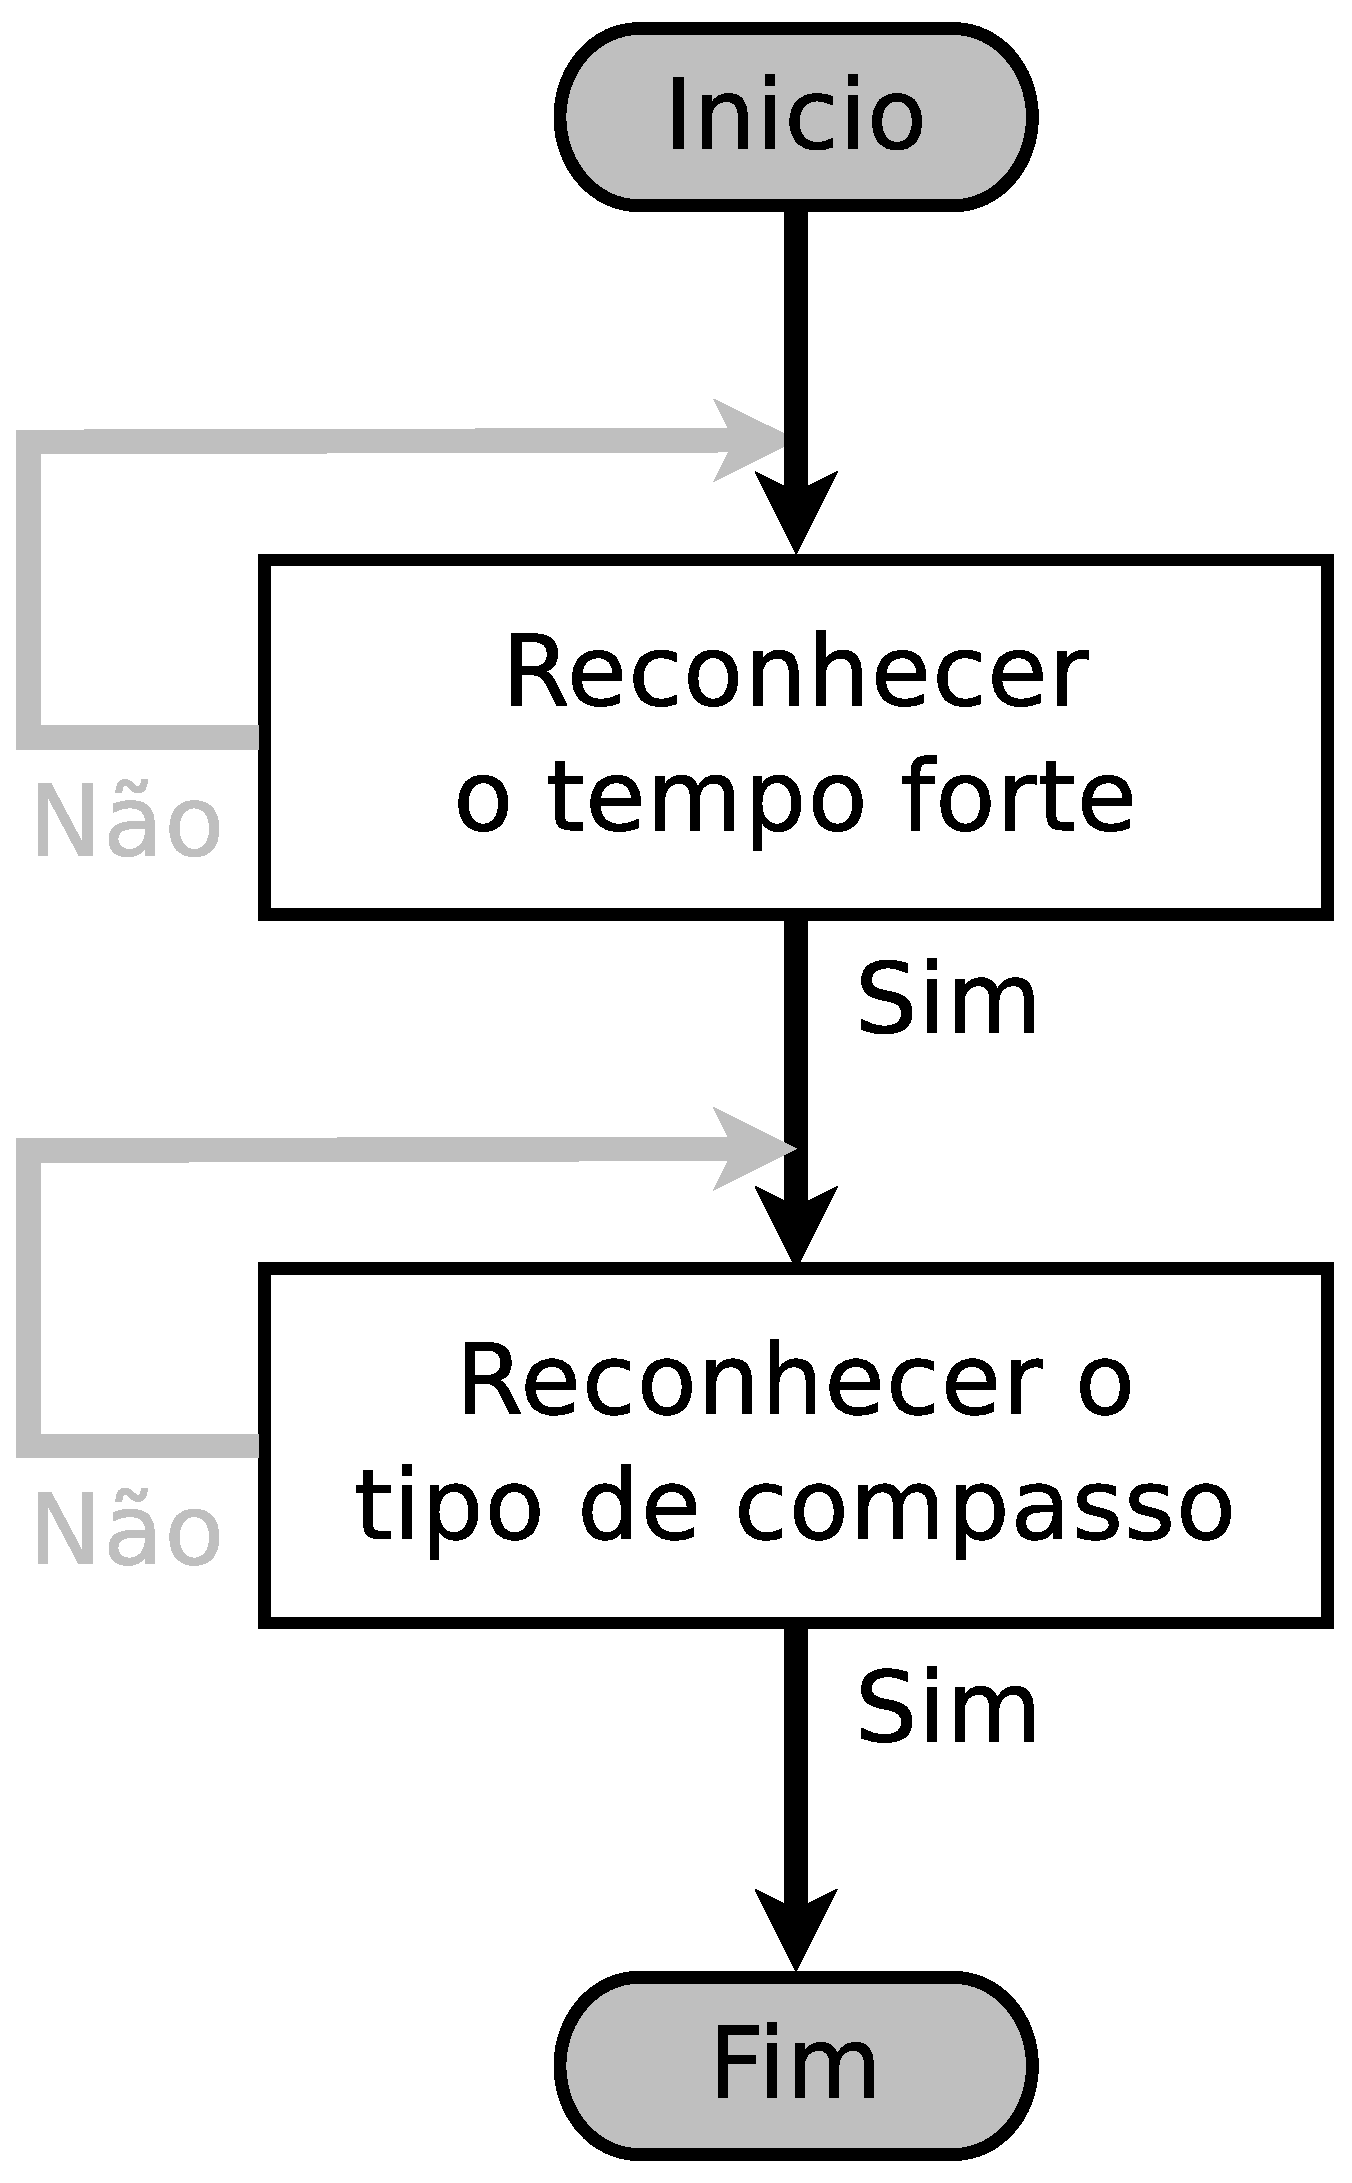
\includegraphics[width=0.65\textwidth]{chapters/cap-musicalidade-percepcion/dancanopulso1.eps}
\caption{Método quase-objetivo.}
\label{fig:fluxodancanopulso1}
\end{subfigure}
~%
\begin{subfigure}[c]{0.45\textwidth}
\centering 
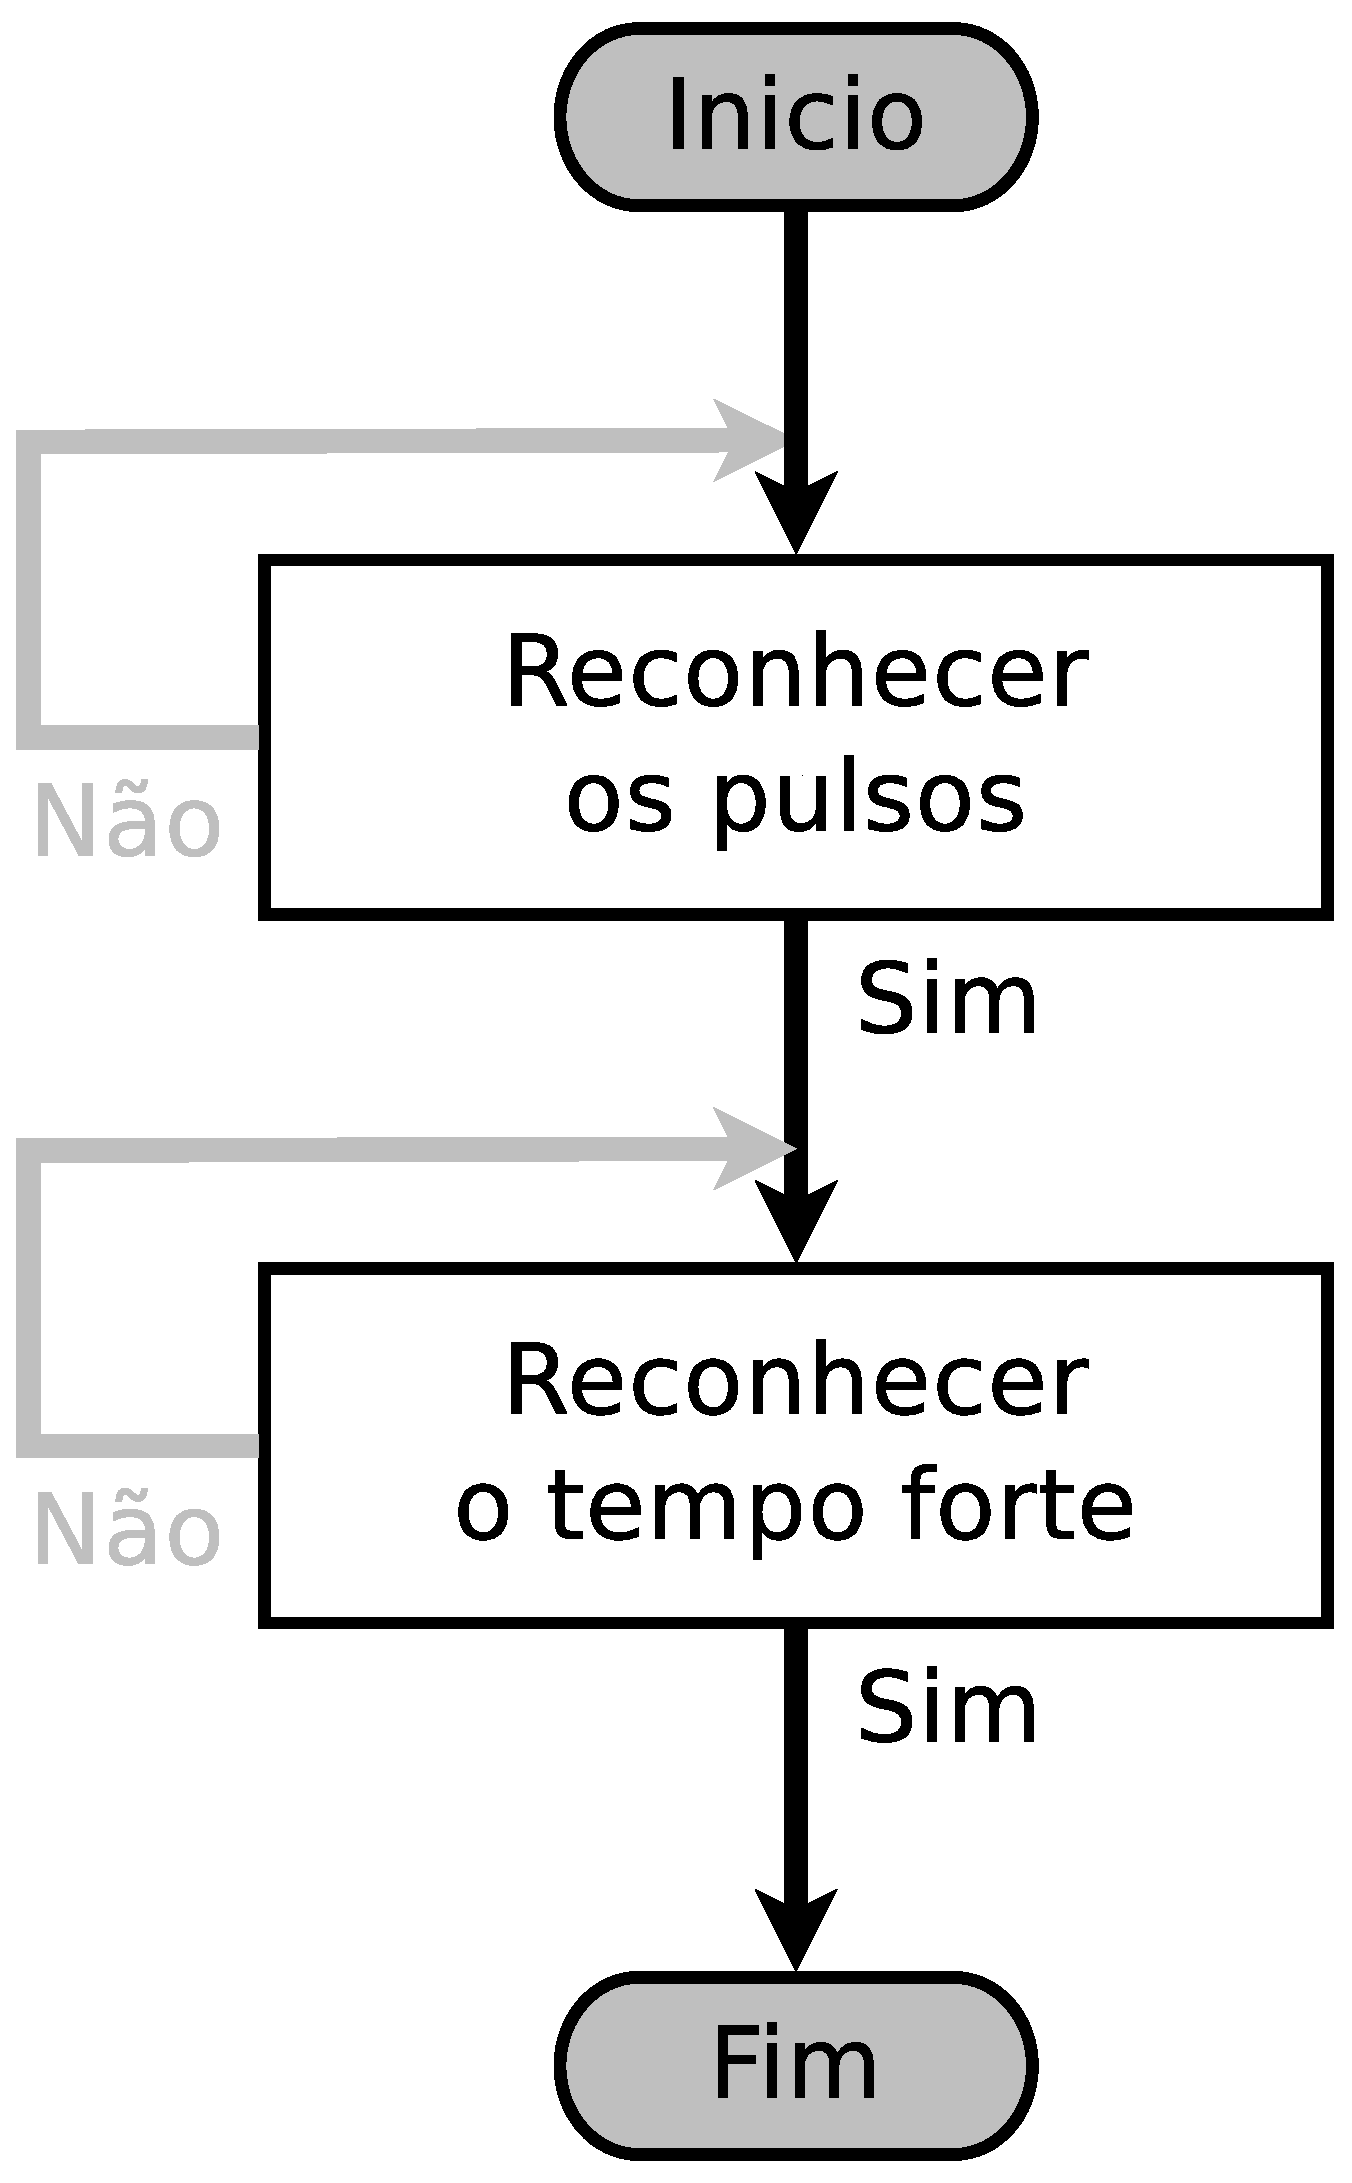
\includegraphics[width=0.65\textwidth]{chapters/cap-musicalidade-percepcion/dancanopulso2.eps}
\caption{Método quase-subjetivo}
\label{fig:fluxodancanopulso2}
\end{subfigure}
    \caption{Percebendo a métrica de uma música}\label{fig:fluxodancanopulso}
\end{figure}



%%%%%%%%%%%%%%%%%%%%%%%%%%%%%%%%%%%%%%%%%%%%%%%%%%%%%%%%%%%%%%%%%%%%%%%%%%%%%%%%
\subsection{Reconhecer o pulso}
\index{Musicalidade!Percepção do pulso}
\label{subsec:perpulsomusica}
As pessoas tendemos a dar palmas ou pisar com o pé, para acompanhar o ritmo da música como um todo,
isto acontece porque inconscientemente percebemos nela um batimento,
continuo e regular, como os batimentos do coração;
assim, quando damos palmas para acompanhar à música, o que estamos 
fazendo e reconhecer o  \hyperref[ref:Pulso]{\textbf{pulso}} musical. 

Este ato está vinculado mais a uma sensação que a um raciocínio,
pelo que é difícil apontar um método para reconhecer o pulso,
que não seja simplesmente indicar que debemos bater palmas ate ``sentir'',
que o pulso das palmas acompanhe ao pulso da música\footnote{Uma
sugestão é fazer isto fechando os olhos para evitar distrações e agudizar os outros sentidos. }.

Porem, sim podemos apontar alguns motivos que inconscientemente nos provocam chegar a este estado de sincronia.
Por exemplo, na Figura \ref{ritmo:procurando-pulso1},
\begin{figure}[!h]
\centering
    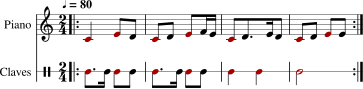
\includegraphics[width=\textwidth]{chapters/cap-musicalidade-percepcion/procurando-pulso1-1.eps}
\caption{Melodia e percussão.}
\label{ritmo:procurando-pulso1}
\end{figure}
podemos ver uma melodia acompanhada por uma percussão,
sendo ``piano'' e ``claves'' escritas usando  \hyperref[subsec:compassobinario]{\textbf{compassos binários}}, 
é dizer com dois tempos, um forte e um fraco, equivalentes cada um à duração de um \hyperref[ref:Pulso]{\textbf{pulso}}.
Assim, se nós fazemos a experiencia de escutar a música descrita na Figura \ref{ritmo:procurando-pulso1},
``sentiremos'' que podemos dar palmas ate sincroniza-nos com o pulso da música\footnote{Oito
palmas em total ate que a música seja reiniciada.}.
Isto é possível, 
a pesar de que em ambos casos as \hyperref[sec:figurasmusicais]{\textbf{figuras musicais}} usadas tem na sua maioria
\hyperref[sec:pos:Duracion]{\textbf{durações}} menores a um tempo;
podemos ver também o uso em menor quantidade de figuras musicais de um tempo de duração,
e só uma vez (no quarto compasso das claves) o uso de uma figura musical maior a um tempo. 
Pelo que podemos afirmar que em media as figuras musicais são menores a um tempo ou um pulso; consequentemente, 
não é esta a informação que usamos inconscientemente para achar o pulso,
devido a que é menor;
mas sim nos dá uma  aproximação do \hyperref[sec:Andamento]{\textbf{andamento}} da música,
aproximação que corrigirmos quando achemos o pulso.
Mas, existem informações que não são perdidas quando usamos figuras musicais menores ou maiores a um pulso,
e estas  são: o \hyperref[def:acentometrico]{\textbf{acento métrico}} e a 
distribuição de \hyperref[eq:acentosubdividio]{\textbf{acentos nas subdivisões de tempos}},
descrita na Pag. \pageref{eq:acentosubdividio}.
Assim, quando uma figura musical  é executada numa subdivisão do tempo, 
esta terá um acento proporcional a esta subdivisão;
por exemplo, uma figura executada na parte fraca do tempo fraco\footnote{Como
a terceira figura musical, do primeiro compasso do piano.}, 
terá um acento menor que uma executada num tempo fraco\footnote{Como
a segunda figura musical, do primeiro compasso do piano.}, 
e uma figura musical executada num tempo fraco terá um acento menor que a de um tempo forte\footnote{Como
a primeira figura musical, do primeiro compasso do piano.}.
Pelo que se deduz, que o que detetamos quando sentimos o pulso, 
é esse fluxo de \hyperref[sec:pos:Intensidade]{\textbf{intensidades}} mudando no tempo, 
como pode ser visto na Figura \ref{ritmo:procurando-pulso2}.
\begin{figure}[!h]
\centering
    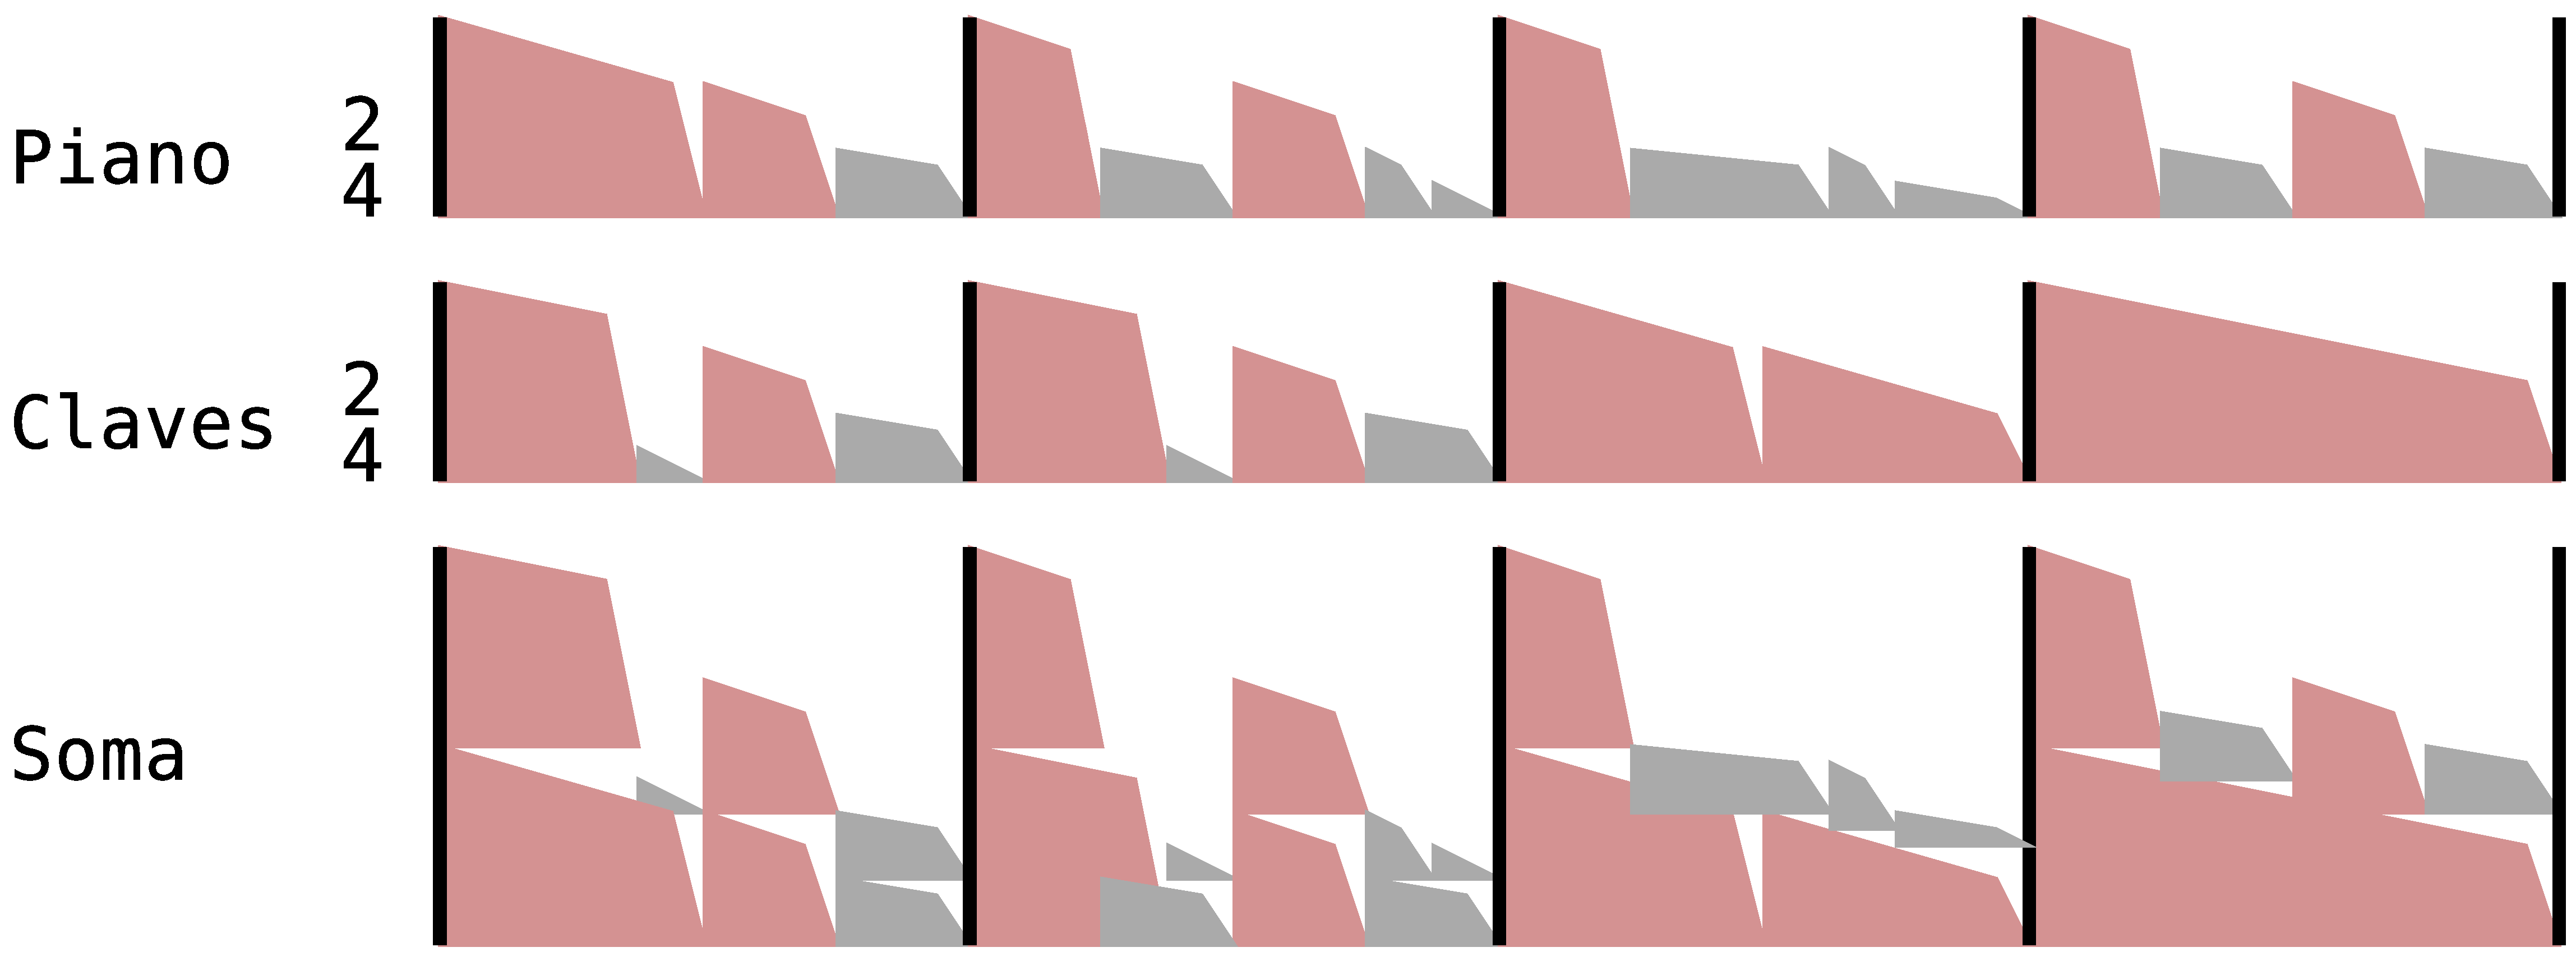
\includegraphics[width=\textwidth]{chapters/cap-musicalidade-percepcion/procurando-pulso2.eps}
\caption{Intensidades na melodia e percussão.}
\label{ritmo:procurando-pulso2}
\end{figure}
Onde temos uma aproximação do diagrama de intensidades: do piano, da clave e da soma de ambos;
no diagrama da ``soma'' fica mais claro porquê inconscientemente detetamos o fluxo de acentos,
e poderíamos inferir que este fluxo ficaria mais próximo ao fluxo do pulso, 
quando aumente o número de instrumentos envolvidos.


%%%%%%%%%%%%%%%%%%%%%%%%%%%%%%%%%%%%%%%%%%%%%%%%%%%%%%%%%%%%%%%%%%%%%%%%%%%%%%%%
\subsection{Reconhecer o tempo forte}
\index{Musicalidade!Tempo forte}
\index{Musicalidade!Bússola}
\label{subsec:perceberTF1}

\begin{wrapfigure}{r}{0.2\textwidth}
  \vspace{-10pt}
  \centering
    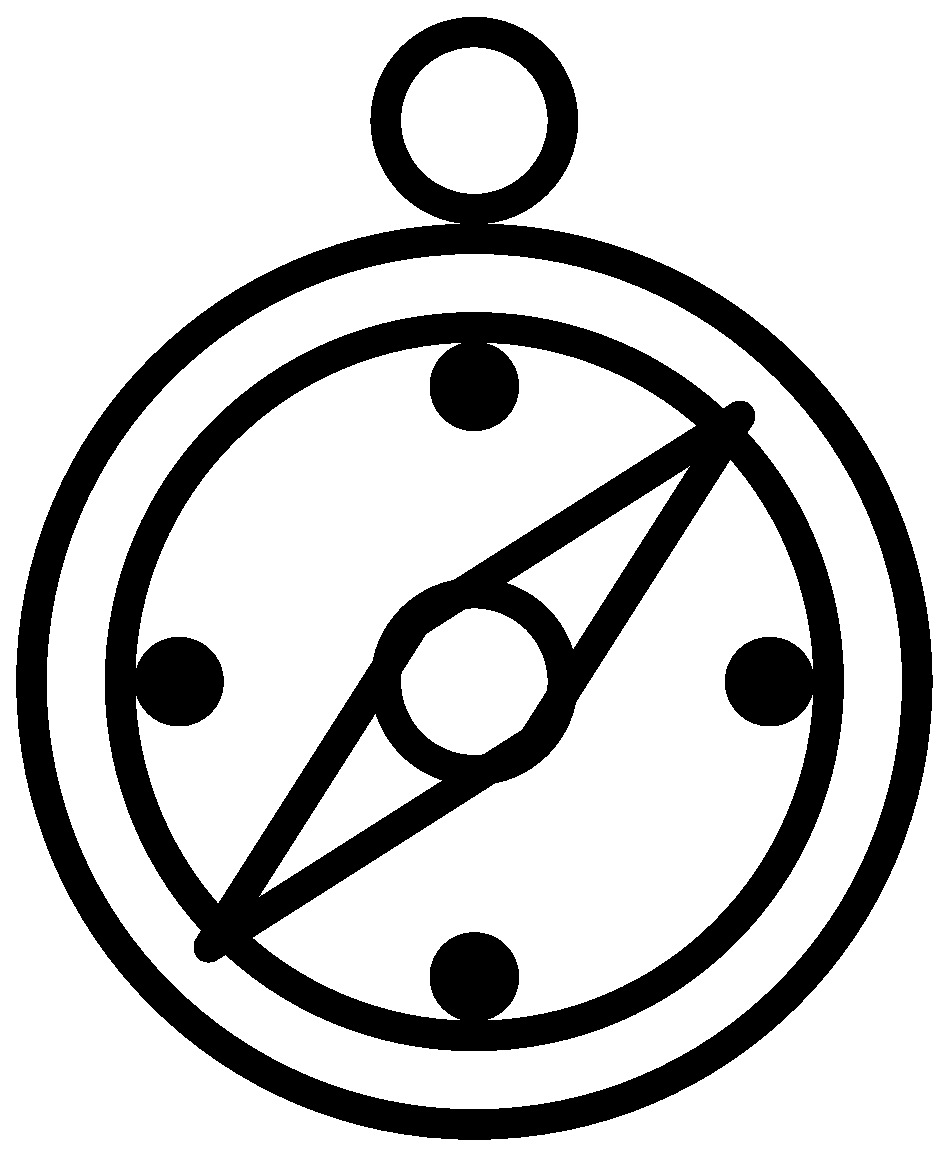
\includegraphics[width=0.15\textwidth]{compass.eps}
  \vspace{-10pt}
\end{wrapfigure}
O tempo forte é o primeiro tempo de cada \hyperref[def:Compasso]{\textbf{compasso}},
este nos ajudará a orientar-nos (bússola) em referencia à métrica da música, 
se precisamos identificá-lo numa música, podemos usar as seguintes informações:
\begin{itemize}
\item O tempo forte é o tempo em que estatisticamente percebemos que as vozes e 
instrumentos convergem executando as notas musicais com maior  \hyperref[sec:pos:Intensidade]{\textbf{intensidade}}  (potencia sonora). 
\end{itemize}

\begin{itemize}
\item Os compositores, seguindo a \hyperref[sec:ProsodiaMusical]{\textbf{prosódia musical}} vista Seção \ref{sec:ProsodiaMusical}, 
geralmente colocam as sílabas tônicas, das palavras, no tempo forte da música  \cite[pp. 149]{medteoria}. 
Da mesma forma, se fazemos um esforço de imaginação e pensamos que os instrumentos ``falam'' ou ``cantam chorando'',
podemos perceber o tempo forte identificando quê ``sílabas'' tem maior intensidade.
\item Se numa música pertencente a alguns dos \hyperref[sec:FamiliaSamba]{\textbf{subgeneros do samba}}, 
conseguimos identificar audivelmente  um padrão de repetição com a onomatopeia ``tchic-tchic tum'', 
então o tum é executado no tempo forte. 
Para mais detalhes ir a Seção \ref{sec:percepcaosamba1}.
\end{itemize}~

Lembremos que esta será uma procura do tempo forte por uma aproximação estatística, 
pois os acentos na música além de estar no tempo forte, 
também aparecem em tempos fracos, nos \hyperref[sec:contratempo]{\textbf{contratempos}}.




Além das indicações anteriores, 
existem outros critérios um pouco mais elaborados para conseguir identificar o tempo forte:
\begin{itemize}
\item Se percebemos um breque (break) na música, 
provocado por uma \hyperref[sec:Frase]{\textbf{frase}} com \hyperref[subsec:FinalAbertoFechado]{\textbf{final fechado}} 
(satisfatório, com uma sensação de ponto final), então este aconteceu no tempo forte.
\item A frase rítmica, das vozes que geram o acompanhamento da melodia principal,
geralmente iniciam no tempo forte; 
o inicio da frase é percebido com uma nota em tempo forte com maior intensidade, 
que a percebida em um tempo forte qualquer\footnote{Pode ser
devido a que se imprime de fato maior intensidade o a que mais instrumentos convergem nesse instante.}.
\end{itemize}

\begin{tcbattention}
É importante ressaltar que na música, 
a melodia principal acentua regularmente seguindo a \hyperref[def:acentometrico]{\textbf{métrica}}
e enfeita acentuando esporadicamente em \hyperref[sec:contratempo]{\textbf{contratempo}}.
Já o acompanhamento percussivo ou harmônico, por sua caraterística regular no padrão do seu ritmo,
geralmente opta por tocar continuamente acentuando no tempo forte,
ou continuamente no contratempo; 
por exemplo na música do reggae o acompanhamento geralmente está a contratempo.
\begin{itemize}
\item ``No Woman No Cry'' de Bob Marley.
\end{itemize}
\end{tcbattention}



%%%%%%%%%%%%%%%%%%%%%%%%%%%%%%%%%%%%%%%%%%%%%%%%%%%%%%%%%%%%%%%%%%%%%%%%%%%%%%%%
\subsection{Reconhecer o tipo de compasso}
\index{Musicalidade!Percepção do tipo de compasso}
\label{subsec:pertipodecompasso}
Se já conseguimos \hyperref[subsec:perceberTF1]{\textbf{identificar o tempo forte}} na música,
então podemos dizer que conhecemos o ciclo de repetição imposto pela métrica,
e podemos predizer quando acontecerá o próximo tempo forte.
Tendo em conta tudo o anterior,
o seguinte passo é deduzir quantos tempos fracos acontecem 
entre um par consecutivo de tempos fortes;
é dizer, 
temos que identificar se a música tem compassos 
\hyperref[subsec:compassobinario]{\textbf{binários}} (2 tempos), 
\hyperref[subsec:compassoternario]{\textbf{ternários}} (3 tempos), 
\hyperref[subsec:compassoquaternario]{\textbf{quaternários}} (4 tempos) 
ou outros. 

Uma forma de deduzir o tipo de compasso utilizado na música  é usando como guia o estilo musical; por exemplo:
\begin{itemize}
\item As músicas dos \hyperref[sec:FamiliaSamba]{\textbf{subgêneros do samba}} 
são principalmente escritas em compassos binários,
porem também é possível ver o uso de compassos quaternários ou de compassos compostos.
\item As músicas de forró comumente usam compassos quaternários,
porem também é possível ver o uso de compassos binários, como no baião. 
\item Em músicas usadas para dançar bolero, salsa, zouk 
e sertanejo universitário é comum perceber o uso de compassos quaternários.
\item Nas músicas onde se dança valsa são usados compassos ternários.
\item etc.
\end{itemize}
Em geral a maioria da música popular ``de moda'', no \AnoLivro, usa uma quantidade par de tempos no compasso;
sendo quaternários em primeiro lugar e binários em segundo.
Pelo que se o estilo musical não é valsa (compassos ternários), 
teremos muito provavelmente um número par de tempos no compasso;
porem, é  pouco provável atualmente achar (na rádio ou em sites de música),
o destaque de músicas em ritmo de valsa.

O método que seguiremos para identificar o tipo de compasso será testar estes tipos,
um a um, ate perceber entre eles uma maior coincidência,
iniciando o teste com o tipo de compasso com mais probabilidade seguindo o estilo musical \cite[pp. 10]{wright1992social}.
Assim, testaremos primeiro os compassos (simples)
\hyperref[subsec:compassobinario]{\textbf{binários}}, 
\hyperref[subsec:compassoternario]{\textbf{ternários}}, 
\hyperref[subsec:compassoquaternario]{\textbf{quaternários}};
se for necessário testaremos alguns compassos compostos 
e em muitas raras ocasiões os compassos mistos.

Não precisamos testar a métrica com a música como um todo,
e sim podemos usar melodias ou ritmos de instrumentos isolados para testar a métrica \cite[pp. 10]{wright1992social};
por exemplo, no caso de musicas com \hyperref[subsec:homofonica]{\textbf{textura homofônica}},
geralmente pela natureza repetitiva e marcada do acompanhamento ou da percussão,
é mais fácil detetar a métrica nessas camadas da música.

\subsubsection{Testando um compasso binário}
A forma mais simples de detetar a métrica dos compassos \hyperref[subsec:compassobinario]{\textbf{binários}},
é fazendo uma troca de peso entre nossos pés (balanço),
ate encaixar o tempo forte\footnote{Para ter certeza de que detetamos o tempo forte, 
podemos usar as técnicas explicadas na Seção \ref{subsec:perceberTF1}.} 
de um lado de nosso balanço,
e perceber que a contagem binária bate com o \hyperref[ref:Pulso]{\textbf{pulso}} da música,
e com uma distribuição de acentos, \{Forte, fraco\};
nesse ponto deduziremos de quê lado do balanço está o tempo forte e o fraco.

\begin{example}[Música com compassos de 2 tempos:]
\label{ex:compassosimples3t}
A música ``Piston de Gafieira'' de Billy Blanco,
está composta por compassos binários (simples), pelo qual tem 2 tempos.
Um exercício interessante, é \hyperref[subsec:perceberTF1]{\textbf{achar o tempo forte}},
por exemplo seguindo as sílabas tônicas na letra da música,
e tentar encaixar a contagem:\{\textbf{1}, 2\}, no ciclo da métrica, acentuando cada tempo 1 (tempo forte). 
\end{example}

\begin{example}[Outros exemplos de compassos binários:]
~
\begin{itemize}
\item ``Tico-Tico no fubá'' de Zequinha de Abreu  \cite[pp. 6]{marcondes1998enciclopedia} \cite[pp. 39,91]{diniz2003almanaque}.
\item ``Brasileirinho'' de Valdir Azevedo  \cite[pp. 133]{perna2002samba}.
\item ``Pelo telefone'' de  Ernesto dos Santos (Donga) e Mauro de almeida.
\item ``Pierrô apaixonado'' de Heitor dos prazeres e Noel Rosa \cite[pp. 1070]{marcondes1977enciclopediav2} \cite[pp. 53]{diniz2008almanaque}.
\item ``A banda'' de Chico Buarque interpretada por Nara Leão \cite[pp. 90]{diniz2008almanaque} \cite{partituraabanda1}.
\end{itemize}
\end{example}


\subsubsection{Testando um compasso ternário}
Neste caso bastará que nós contemos ate 3, iniciando em 1 no tempo forte,
e procurando que os três tempos encaixem perfeito no ciclo da métrica (entre dois tempos fortes consecutivos).
Se percebemos que esta contagem encaixa na métrica,
com uma distribuição de acentos, \{Forte, fraco, fraco\} \cite[pp. 10]{wright1992social}, 
então estamos sim, frente a um  \hyperref[subsec:compassoternario]{\textbf{compasso ternário}}.

\begin{example}[Música com compassos de 3 tempos:]
\label{ex:compassosimples3t3}
A música ``João e Maria'' de Chico Buarque,
está composta por compassos ternários (simples), pelo qual tem 3 tempos.
Um exercício interessante, é \hyperref[subsec:perceberTF1]{\textbf{achar o tempo forte}},
por exemplo seguindo as sílabas tônicas na letra da música,
e tentar encaixar a sequencia:\{\textbf{1}, 2 , 3\}, no ciclo da métrica,acentuando cada tempo 1 (tempo forte). 
\end{example}

\begin{example}[Outros exemplos de compassos ternários:]
\label{ex:compassosimples3t2}
~
\begin{itemize}
\item ``Rio grande tchê'' interpretado pelo grupo Os serranos.
\item ``Blusa Vermelha'' interpretado pelo Trio Parada Dura.
%\item ``Ainda ontem chorei de saudade'' interpretado por Eduardo Costa e Leonardo.
\item ``Último adeus'' interpretado por Eduardo Costa e Leonardo.
\item ``Chao de Giz'' de Ze Ramalho.
\end{itemize}
\end{example}

\subsubsection{Testando um compasso quaternário}
Neste caso nos temos que contar ate 4, iniciando em 1 no tempo forte,
e procurando que os quatro tempos encaixem perfeito no ciclo da métrica.
Se percebemos que esta contagem encaixa na métrica (entre dois tempos fortes consecutivos),
com uma distribuição de acentos, \{Forte, fraco, meio forte, fraco\} \cite[pp. 10]{wright1992social}, 
então estamos sim, frente a um  \hyperref[subsec:compassoquaternario]{\textbf{compasso quaternário}}.


\begin{example}[Música com compassos de 4 tempos:]
\label{ex:compassosimples4t}
A música (\hyperref[subsec:marcha]{\textbf{Marcha}}) ``Noite dos Mascarados'' de Chico Buarque,
está composta por compassos quaternários (simples), pelo qual tem 4 tempos,
e podemos contar: \{\textbf{1}, 2 , 3, 4\}, acentuando cada tempo 1 (tempo forte) e cada tempo 3 (tempo semi forte).
Um exercício interessante, é \hyperref[subsec:perceberTF1]{\textbf{achar o tempo forte}},
por exemplo seguindo as sílabas tônicas na letra da música,
e tentar encaixar a sequencia da contagem no ciclo da métrica, 
\end{example}

\begin{example}[Outros exemplos de compasso quaternário:]
~
\begin{itemize}
\item ``Sambolero'' interpretado por Luiz Bonfá \cite[pp. 49]{sambolero}.
\item ``Cê que sabe'' interpretado por Cristiano Araujo.
\item ``Vai dar namoro'' interpretado por Bruno e Marrone.
\item ``Vou te amarrar a minha cama'' interpretado por Bruno e Marrone.
\item ``Borbulhas de amor'' interpretado por Eduardo costa e Leonardo%Gustavo Lima.
\end{itemize}
\end{example}

\subsubsection{Compassos compostos}
Na prática, bastará a principio, para um dançarino iniciante,
reconhecer os compassos \hyperref[subsec:compassoquaternario]{\textbf{quaternários}}, 
\hyperref[subsec:compassobinario]{\textbf{binários}}, e 
\hyperref[subsec:compassoternario]{\textbf{ternários}},
nesse ordem de ocorrência;
pois as raras ocasiões onde estejamos frente a um \hyperref[sec:compaso]{\textbf{compasso composto}},
um dançarino pode tratar ele como sua contraparte simples,
e desenvolver-se suficientemente bem na dança. 
Podemos perceber o uso de compassos compostos de 6 pulsos nos Exemplos \ref{ex:compassocomposto6}
e \ref{ex:compassocomposto6b},
este tipo de compassos é muito comum nas baladas pop e na música erudita.
\begin{example}[Música com compassos de 6 pulsos:]
\label{ex:compassocomposto6}
Um exemplo deste tipo de música pode ser escutado em ``A Thousand Years'', 
interpretado por Christina Perri. É fácil perceber como podemos nos confundir,
pensando que a música usa compassos binários (simples) de andamento lento,
ou ternários de andamento rápido; quando na realidade trata-se de compassos binários compostos de 6 pulsos (dois tempos),
possivelmente com formula de compasso 6/8.

Um dançarino, mesmo sabendo que trata-se de um \hyperref[compasso:binario]{\textbf{compasso binário composto}} (de 6 pulsos),
pode tratar a música como se esta fosse binária simples, e dançar em grupos de dois passos lentos,
ou como se fosse ternaria simples, e tentar dançar estilo valsa porem muito rápida.

A mínima subdivisão a ser feita por nós na dança, 
será a de assumir um compasso binário, usando movimentos binários,
pois quando tentemos subdividir por dois um passo, para encaixar um ``tchic tchic tum'',
acharemos a dança desconfortável, devido a que
entraremos em conflito com o \hyperref[ref:Pulso]{\textbf{pulso}}, 
que divide o compasso em porções múltiplos de três.
  
\end{example}

\begin{example}[Outros exemplos de compassos binários de 6 pulsos:]
\label{ex:compassocomposto6b}
~
\begin{itemize}
\item ``Quem é ela'' interpretado por Marco e Mário.
\item ``Seu amor ainda é tudo'' interpretado por Eduardo Costa e Leonardo.
\item ``You don't own me'' interpretado por Grace.
\item ``We are the champions'' interpretado pelo grupo Queen.
\item ``Hallelujah'' interpretado por Rufus Wainwright.
\item ``Happy Christmas'' interpretado por John Lennon.
\item ``The House of the Rising Sun'' interpretado pelo grupo  The Animals.
%\item ``Lakmé'' interpretado por Léo Délibes.
%\item ``Nothing Else Matters'' interpretado pelo grupo Metallica.
\end{itemize}
\end{example}

\subsubsection{Compassos mistos}
Em muitas raras ocasiões, mais raro ainda que o caso dos compassos compostos, 
podemos achar compassos mistos, como nos Exemplos \ref{ex:compassomisto5} e \ref{ex:compassomisto7}.

\begin{example}[Música com compassos de 5 pulsos:]
\label{ex:compassomisto5}
A música ``Take Five'' interpretada por  Dave Brubeck,
está composta por compassos mistos (alternados), criados pela concatenação de um compasso binário e um ternário,
contando-se os tempos: \{\textbf{1}, 2, \textbf{1}, 2, 3\}, acentuando o 1.
Um exercício interessante, é achar o tempo forte  e tentar encaixar esta sequencia na música, 
\end{example}

\begin{example}[Música com compassos de 7 pulsos:]
\label{ex:compassomisto7}
A música ``Money'' interpretada pela banda  Pink Floyd,
esta composta por compassos mistos (alternados), criados pela concatenação de um compasso quaternário e um ternário,
contando-se os tempos: \{\textbf{1}, 2 , 3, 4, \textbf{1}, 2, 3\}, acentuando cada tempo 1 e o primeiro 3 (meio forte).
Um exercício interessante, é achar o tempo forte  e tentar encaixar esta sequencia na música, 
\end{example}
